\documentclass{beamer}
\usepackage{graphics,amssymb,amsfonts,amsmath}
\usepackage{pgf,tikz}
\usetikzlibrary{shapes,shapes.geometric,trees,positioning,fit,backgrounds}
\DeclareGraphicsExtensions{.jpg,.pdf,.mps,.png}
\usepackage[utf8]{inputenc}
\usepackage[brazil]{babel}
\usepackage[normalem]{ulem}
\usepackage{standalone}
\usepackage{pgfpages,enumerate,hyperref}
\usepackage{palatino}   %Fonte sem serifa.
\usepackage{ragged2e}   %Par\'agrafo justificado.
\usepackage{minted}
\usepackage{tikz}
% \usetheme{CambridgeUS}
% \usetheme{AnnArbor}
% \usecolortheme{lily}
\usecolortheme{orchid}
\usefonttheme[onlymath]{serif}

\def\theFancyVerbLine{%
  \rmfamily\tiny\arabic{FancyVerbLine}%
  {\tikz[remember picture,overlay]\node(minted-\arabic{FancyVerbLine}){};}%
}

\tikzstyle{box}=[draw, minimum width=2cm, minimum height=1cm, node distance=1.3cm, rounded corners]

%colocando n\'umero de p\'aginas no slide.
\setbeamertemplate{footline}[frame number]

% desativando os botoes de navegacao.
\beamertemplatenavigationsymbolsempty

%Tela cheia
\hypersetup{pdfpagemode=FullScreen}

% Layout da p\'agina
\hypersetup{pdfpagelayout=SinglePage,urlcolor=blue,colorlinks=true}

\definecolor{terminalcolor}{RGB}{48,10,36}

% Ambiente bash
\newminted{bash}{bgcolor=terminalcolor,formatcom=\color{white}}

% Ambiente python
\newminted{python}{bgcolor=green!25!white,linenos}

% Ambiente html
\newminted{html}{bgcolor=cyan!25}

\tikzstyle{every node}=[anchor=west]
\tikzstyle{selected}=[draw=red,fill=green!30]
\tikzstyle{optional}=[dashed,fill=gray!50]

\title{Tutorial Django\\ Introdução simples}
\author{R\'egis da Silva\\ {\texorpdfstring{\color{blue}}{ }about.me/rg3915}}
\institute{\url{github.com/grupy-sp/encontros}}
\date{27 de Janeiro de 2016}

\begin{document}
\justifying %Par\'agrafo justificado.

%Neste caso insere somente no primeiro slide.
{%
%\usebackgroundtemplate{\centering \vspace*{5cm} \includegraphics[width=\paperwidth]{figuras/djangoPython}}

% \usebackgroundtemplate{%
% \vbox to \paperheight{\vfil\hbox to \paperwidth{\hfil
\includegraphics[width=\paperwidth]{img/logo_mascote.jpg}\hfil}\vfil}
% }

% \begin{frame}

% \end{frame}
% }

\begin{frame}
	\titlepage
\end{frame}

\begin{frame}[fragile]\frametitle{Script}

\begin{bashcode}
$ wget --output-document=setup.sh link
$ source setup.sh myproject
\end{bashcode}

\end{frame}


\begin{frame}\frametitle{Objetivo}
	\begin{itemize}
        \item Criar a view mais simples do mundo
        \item Criar um cadastro de pessoas
        \item Editar os dados pelo Admin
	\end{itemize}
\end{frame}

\begin{frame}\frametitle{O que \'e Django?}

Segundo Django Brasil,

\

\begin{exampleblock}{}
    {\it Django \'e um framework web de alto n\'ivel escrito em Python que estimula o desenvolvimento r\'apido e limpo.}
\end{exampleblock}

\end{frame}

\begin{frame}\frametitle{O que \'e Django?}

\begin{itemize}[<+(1)->]
    \item adota o padr\~ao MTV
    \item possui ORM
    \item admin
    \item heran\c ca de templates e modelos
    \item open source
\end{itemize}

\end{frame}

\begin{frame}\frametitle{Versão atual (Jan/16)}

    \begin{center}
    \Huge Django==1.9.1
    \end{center}

\end{frame}


\begin{frame}\frametitle{Sites}

\begin{enumerate}
    \item \url{www.djangoproject.com/}

    \item \url{www.djangopackages.com/}

    \item \url{tutorial.djangogirls.org/pt/index.html}

    \item \url{www.groups.google.com/forum/django-brasil}

    \item \url{www.pythonclub.com.br/}

    \item \url{www.realpython.com/blog/categories/django/}
\end{enumerate}

\end{frame}


\begin{frame}[fragile]\frametitle{Instalação}

\begin{bashcode}
$ virtualenv -p python3 .venv
$ source .venv/bin/activate
$ pip install django
\end{bashcode}

\end{frame}

\begin{frame}[fragile]\frametitle{Criando o Projeto}

\begin{bashcode}
$ django-admin.py startproject myproject .
\end{bashcode}

\end{frame}

\begin{frame}[fragile]\frametitle{Criando a App}

\begin{bashcode}
$ python manage.py startapp core
\end{bashcode}

\end{frame}

\begin{frame}[fragile]

\begin{tikzpicture}[%
  grow via three points={one child at (0.5,-0.7) and
  two children at (0.5,-0.7) and (0.5,-1.4)},
  edge from parent path={(\tikzparentnode.south) |- (\tikzchildnode.west)}]
  \node {.}
    child { node {manage.py}}
    child { node [selected] {myproject}
      child { node {\_\_init\_\_.py}}
      child { node [optional] {settings.py}}
      child { node [optional] {urls.py}}
      child { node {wsgi.py}}
      child { node [selected] {core}
        child { node [optional] {admin.py}}
        child { node {\_\_init\_\_.py}}
        child { node [optional] {models.py}}
        child { node [optional] {tests.py}}
        child { node [optional] {views.py}}
      }
    };
\end{tikzpicture}

\end{frame}

\begin{frame}

\begin{tikzpicture}
    \node[box,fill=blue!25] (a) {Admin};
    \node[box,fill=yellow!50] (v) [right = of a] {Views};
    \node[box,fill=orange!50] (u) [right = of v] {Urls};
    \node[box,fill=green!40] (m) [above = of v.north west] {Models};
    \node[box,fill=cyan!50] (f) [right = of m] {Forms};
    \node[box,fill=green!25] (t) [below = of u] {Templates};
    \node[box,fill=green!25] (i) [below = of t, yshift=.7cm] {index.html};
    \node (tdd) [below = of a,yshift=-2.5cm] {Tests};
    \node[box,fill=gray!25] [left = of tdd] {Settings};
    \draw(v) to[out=0, in=170] (u);
    \draw(v) to[out=90, in=-90] (m);
    \draw(v) to[out=90, in=-90] (f);
    \draw(m) to[out=0, in=180] (f);
    \draw[dashed](v) to[out=-90, in=90] (t);
    \draw(u) to[out=-100, in=80] (t);
    \draw(t) to[out=-90, in=90] (i);
    \draw(a) to[out=0, in=180] (m);
    \draw(a) to[out=10, in=180] (v);
    \draw(a) to[out=-20, in=215] (u);

    \begin{pgfonlayer}{background}
        \node [draw,rounded corners,fill=teal!20,fit=(a) (m) (u) (i)] {};
    \end{pgfonlayer}

\end{tikzpicture}

\end{frame}

\begin{frame}[fragile]\frametitle{Django funcionando em n\'ivel 0}

Criando a primeira migra\c c\~ao

\begin{bashcode}
$ python manage.py migrate
\end{bashcode}

\

\
\pause
Rodando o projeto

\begin{bashcode}
$ python manage.py runserver
\end{bashcode}

\

\

Por padr\~ao ele est\'a rodando na porta 8000

\url{http://localhost:8000/} ou \url{http://127.0.0.1:8000/}
\pause
ou

\begin{bashcode}
$ python manage.py runserver <PORTA>
$ python manage.py runserver 8080
\end{bashcode}

\url{http://localhost:8080/}
\end{frame}


\begin{frame}

    \begin{figure}[h]
      \centering
        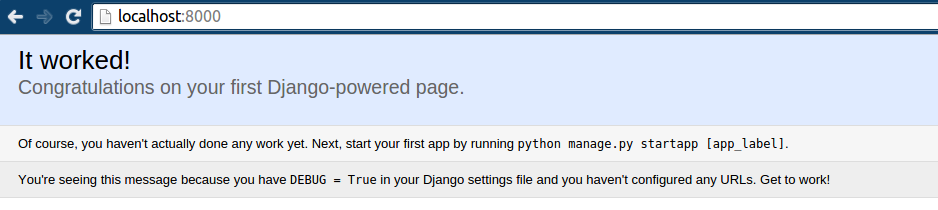
\includegraphics[width=\paperwidth]{img/it_worked.png}
    \end{figure}

\end{frame}


\begin{frame}\frametitle{O m\'inimo - n\'ivel 1: settings, views, urls}

\begin{tikzpicture}[%
  grow via three points={one child at (0.5,-0.7) and
  two children at (0.5,-0.7) and (0.5,-1.4)},
  edge from parent path={(\tikzparentnode.south) |- (\tikzchildnode.west)}]
  \node {.}
    child { node [selected] {myproject}
      child { node {...} }
      child { node {settings.py}}
      child { node {urls.py}}
      child { node [selected] {core}
        child { node {...} }
        child { node {views.py}}
      }
    };
\end{tikzpicture}

\end{frame}


\begin{frame}[fragile]\frametitle{Editando settings.py}

\begin{pythoncode}
INSTALLED_APPS = (
    ...
    'myproject.core',
)
\end{pythoncode}

\end{frame}


\begin{frame}[fragile]\frametitle{A view mais simples do mundo}

\begin{pythoncode}
# from django.shortcuts import render
from django.http import HttpResponse

def home(request):
    return HttpResponse('<h1>Django</h1>
                         <h3>Bem vindo ao Grupy-SP</h3>')
\end{pythoncode}

\end{frame}


\begin{frame}[fragile]\frametitle{Editando urls.py}

\begin{pythoncode}
from django.conf.urls import url
import myproject.core.views as v

urlpatterns = [
    url(r'^$', v.home),
]
\end{pythoncode}

\end{frame}

\begin{frame}

    \begin{figure}[h]
      \centering
        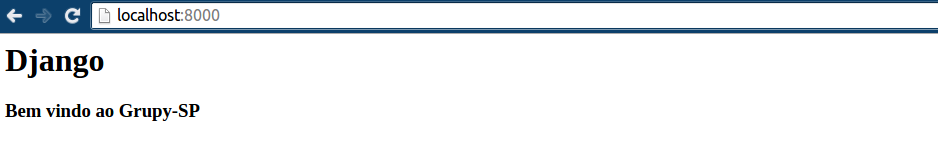
\includegraphics[width=\paperwidth]{img/HttpResponse.png}
    \end{figure}

\end{frame}


\begin{frame}[fragile]\frametitle{Tocando o barco}

\textbf{Editando settings.py}

\begin{pythoncode}
LANGUAGE_CODE = 'pt-br'

TIME_ZONE = 'America/Sao_Paulo'
\end{pythoncode}


\end{frame}



\begin{frame}[fragile]\frametitle{Editando views.py}

\begin{pythoncode}
from django.shortcuts import render
# from django.http import HttpResponse

# def home(request):
#     return HttpResponse('<h1>Django</h1><h3>Bem vindo ao Grupy-SP</h3>')

def index(request):
    return render(request, 'index.html')
\end{pythoncode}


\end{frame}

\begin{frame}[fragile]\frametitle{Editando urls.py}

\begin{pythoncode}
from django.conf.urls import url
import myproject.core.views as v
from django.contrib import admin

urlpatterns = [
    url(r'^$', v.home),
    url(r'^index/$', v.index),
    url(r'^admin/', admin.site.urls),
]
\end{pythoncode}


\end{frame}


\begin{frame}\frametitle{A pasta templates}

\begin{tikzpicture}[%
  grow via three points={one child at (0.5,-0.7) and
  two children at (0.5,-0.7) and (0.5,-1.4)},
  edge from parent path={(\tikzparentnode.south) |- (\tikzchildnode.west)}]
  \node [selected] {myproject}
      child { node {...}}
      child { node {settings.py}}
      child { node {urls.py}}
      child { node [selected] {core}
        child { node {...}}
        child { node {views.py}}
          child { node [selected] {templates}
          child { node {index.html}}
        }
  };
\end{tikzpicture}

\end{frame}

\begin{frame}

    \begin{figure}[h]
      \centering
        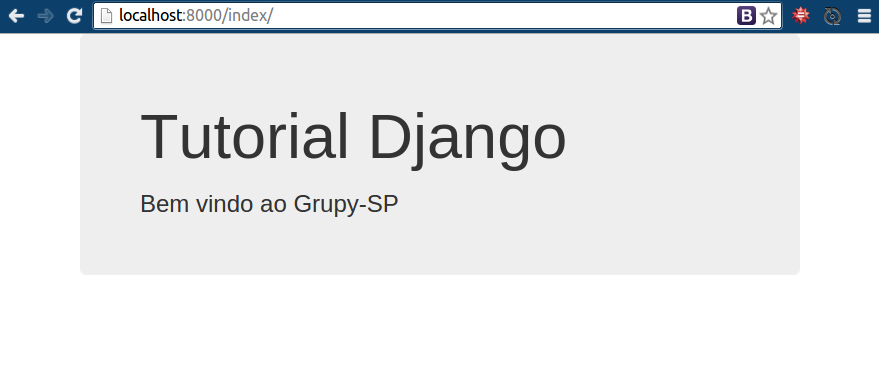
\includegraphics[width=\paperwidth]{img/index.png}
    \end{figure}

\end{frame}


\begin{frame}[fragile]\frametitle{Editando models.py}

\begin{pythoncode}
from django.db import models

class Person(models.Model):
    first_name = models.CharField('nome', max_length=50)
    last_name = models.CharField('sobrenome', max_length=50)
    phone = models.CharField('telefone', max_length=20, blank=True)
    email = models.EmailField('e-mail', blank=True)
    blocked = models.BooleanField('bloqueado', default=False)
    created = models.DateTimeField('criado em', auto_now_add=True)

    class Meta:
        ordering = ['first_name']
        verbose_name = 'pessoa'
        verbose_name_plural = 'pessoas'

    def __str__(self):
        return ' '.join(self.first_name, self.last_name)
\end{pythoncode}

\end{frame}

\begin{frame}\frametitle{Tipos de campos}
  \begin{center}
    \large https://docs.djangoproject.com/en/1.9/ref/models/fields/
  \end{center}
\end{frame}

\begin{frame}[fragile]\frametitle{Editando o admins.py}

\begin{pythoncode}
from django.contrib import admin
from myproject.core.models import Person

admin.site.register(Person)
\end{pythoncode}

\end{frame}

\begin{frame}[fragile]\frametitle{Editando o admins.py}

\begin{pythoncode}
from django.contrib import admin
from myproject.core.models import Person

class PersonModelAdmin(admin.ModelAdmin):
    list_display = ('__str__', 'phone', 'email',
                    'blocked', 'created')
    search_fields = ('first_name', 'last_name',
                     'phone', 'email')
    list_filter = ('blocked',)

admin.site.register(Person, PersonModelAdmin)
\end{pythoncode}

\end{frame}

\begin{frame}[fragile]\frametitle{Atualizando o banco}

\begin{bashcode}
$ python manage.py makemigrations
$ python manage.py migrate
\end{bashcode}

\end{frame}

\begin{frame}[fragile]\frametitle{Criando um super usuário}

\begin{bashcode}
$ python manage.py createsuperuser
\end{bashcode}

\end{frame}


\begin{frame}

    \begin{figure}[h]
      \centering
        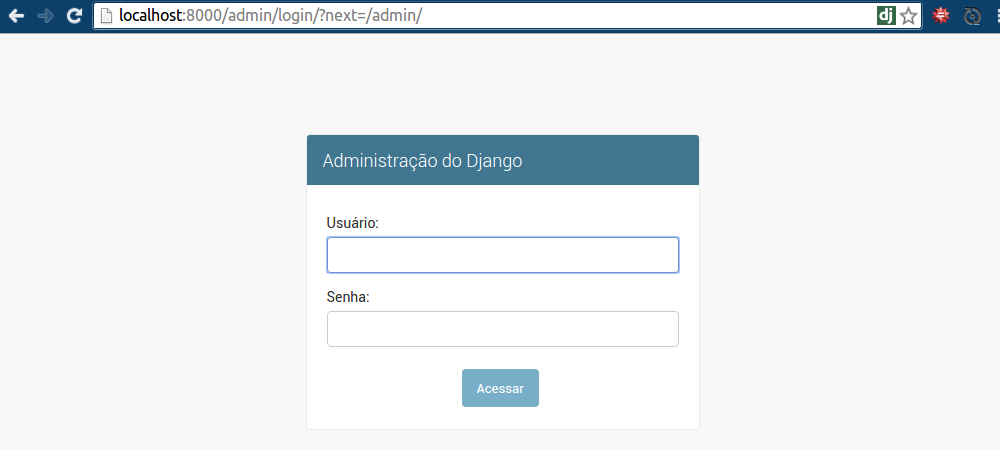
\includegraphics[width=\paperwidth]{img/admin1.png}
    \end{figure}

\end{frame}



\begin{frame}

    \begin{figure}[h]
      \centering
        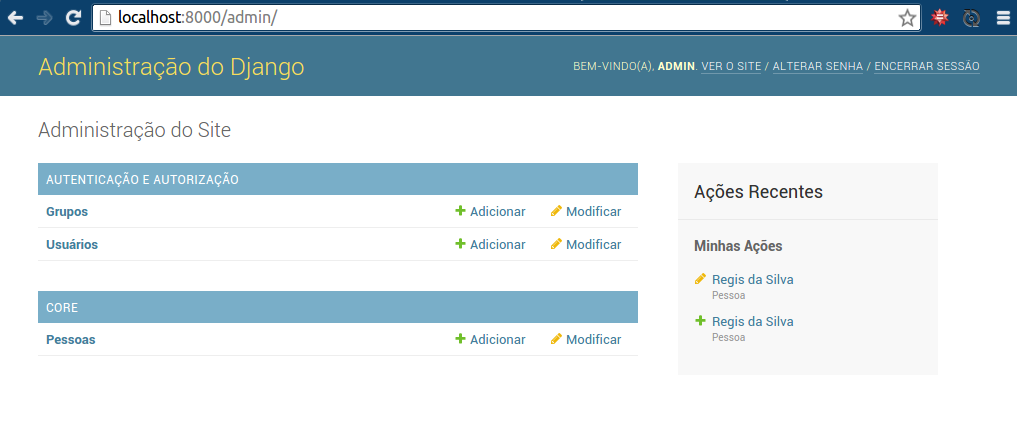
\includegraphics[width=\paperwidth]{img/admin2.png}
    \end{figure}

\end{frame}



\begin{frame}

    \begin{figure}[h]
      \centering
        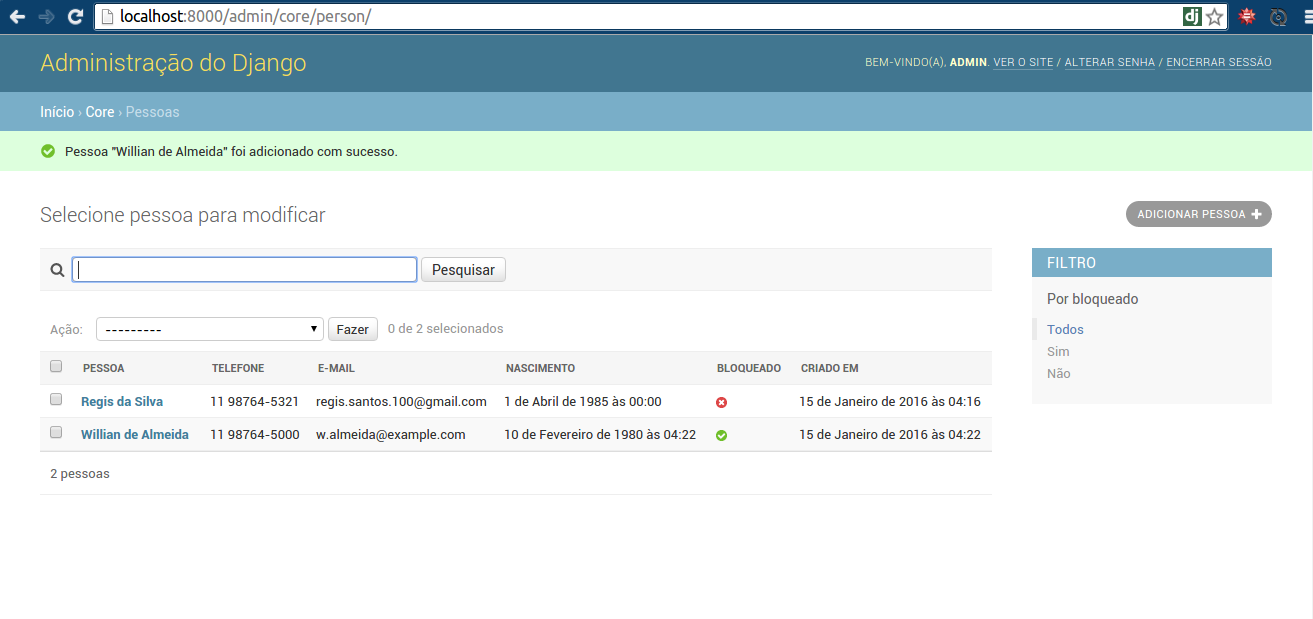
\includegraphics[width=.9\paperwidth]{img/admin3.png}
    \end{figure}

\end{frame}



\begin{frame}

    \begin{figure}[h]
      \centering
        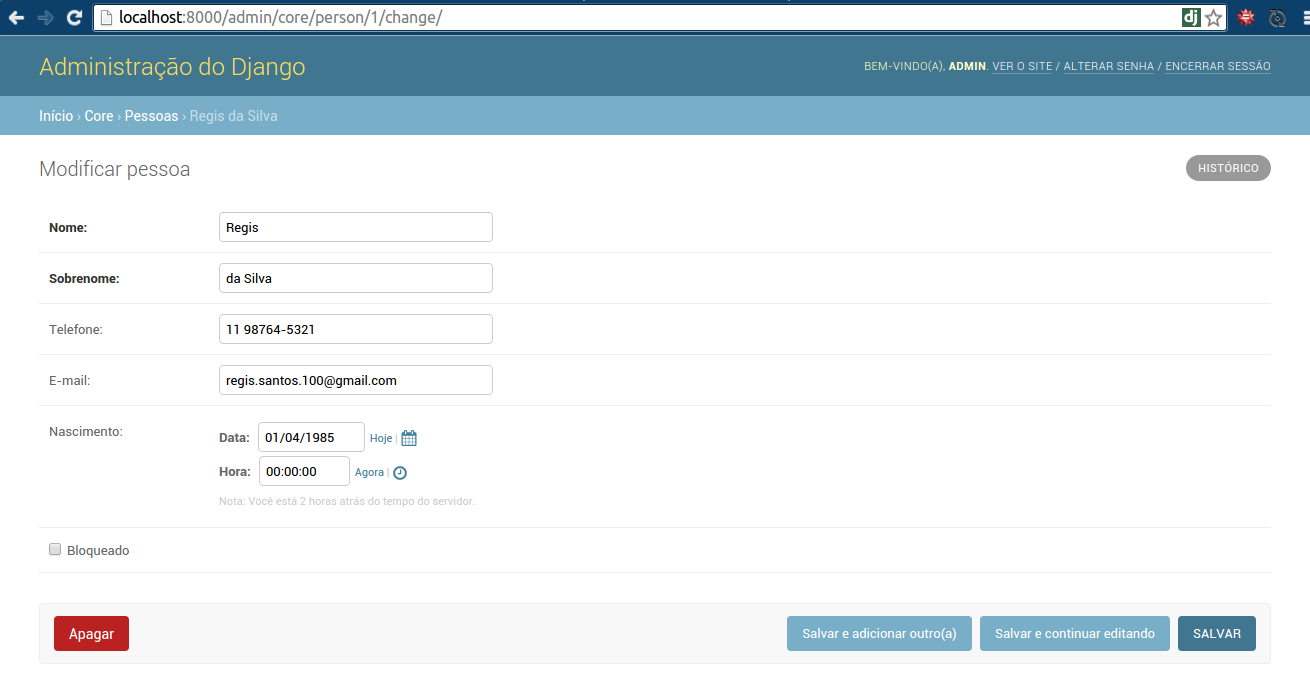
\includegraphics[width=.9\paperwidth]{img/admin4.png}
    \end{figure}

\end{frame}


\begin{frame}
	\centering
	\huge Obrigado!

	\

	\

	\large Dúvidas?
\end{frame}

\begin{frame}
	\titlepage
\end{frame}

\end{document}